\section{Benchmark signal models}
\label{sec:models}

We consider two simplified models with bottom squark pair production, both
resulting in a $\PH$+jets final state.
% In both cases, we assume bottom
%squark as a reference, even if there is no explicit use of b-jet
%tagging in the CMS analysis. Since there is no …, the results generalize to generic squarks. 

In the first model, hereafter referred to as model A, we consider the
asymmetric production of a $\sbottom_2
\sbottom_1$ pair, where $\sbottom_2$ and $\sbottom_1$ are the heaviest
and the lightest bottom squarks, respectively. The $\sbottom_2$ decays
to $\cPqb \chiztwo$, with $\chiztwo \to \PH \chizone$. The lightest neutralino $\chizone$ is
assumed to be the LSP. The $\sbottom_1$, close in mass to the LSP,
decays to $\cPqb \chizone$. All the other SUSY partners are assumed to be
too heavy to be produced at the LHC and are ignored in this
analysis. This model represents a new mechanism for the production of
$\PH+2\cPqb\textrm{-}\mathrm{jets}+\mathrm{invisible}$, with one of
the associated \cPqb-jets typically having low momentum.

In the second model, hereafter referred to as model B~\cite{annthesis}, two bottom
squarks $\sbottom_1\sbottom_1$ are produced, each decaying as
$\sbottom_1 \to \cPqb \chiztwo$. The $\chiztwo$ then decays to $\PH
\chizone$, the $\chizone$ being the LSP. As for model A, the other SUSY
partners are ignored. This simplified model corresponds to a final
state consisting of $2\PH+2\cPqb\textrm{-}\mathrm{jets}+\mathrm{invisible}$.

The mass spectrum for each model is shown in
Fig.~\ref{fig:simplifiedModels}. We fix the $\chiztwo$ and $\chizone$ masses to 230\GeV
and 100\GeV, respectively.  In model A, %three benchmarks are
%assumed for the $\sbottom_1$ mass: 130\GeV, 165\GeV, and 200\GeV. 
we fix the $\sbottom_1$ mass to 130\GeV as varying its mass
in between the limits of the $\chizone$ and $\chiztwo$ masses has little effect.
Finally, we scan the $\sbottom_2$ ($\sbottom_1$) mass between 250\GeV
and 800\GeV for model A (B). These assumptions do not limit the
conclusions derived on the squark production cross section. In fact,
the analysis is sensitive to mass differences and not to the absolute
mass of SUSY partners. On the other hand, the chosen LSP and NLSP
masses does play a role when the cross section limits are
translated in terms of mass exclusion bounds.


\begin{figure}[htb]
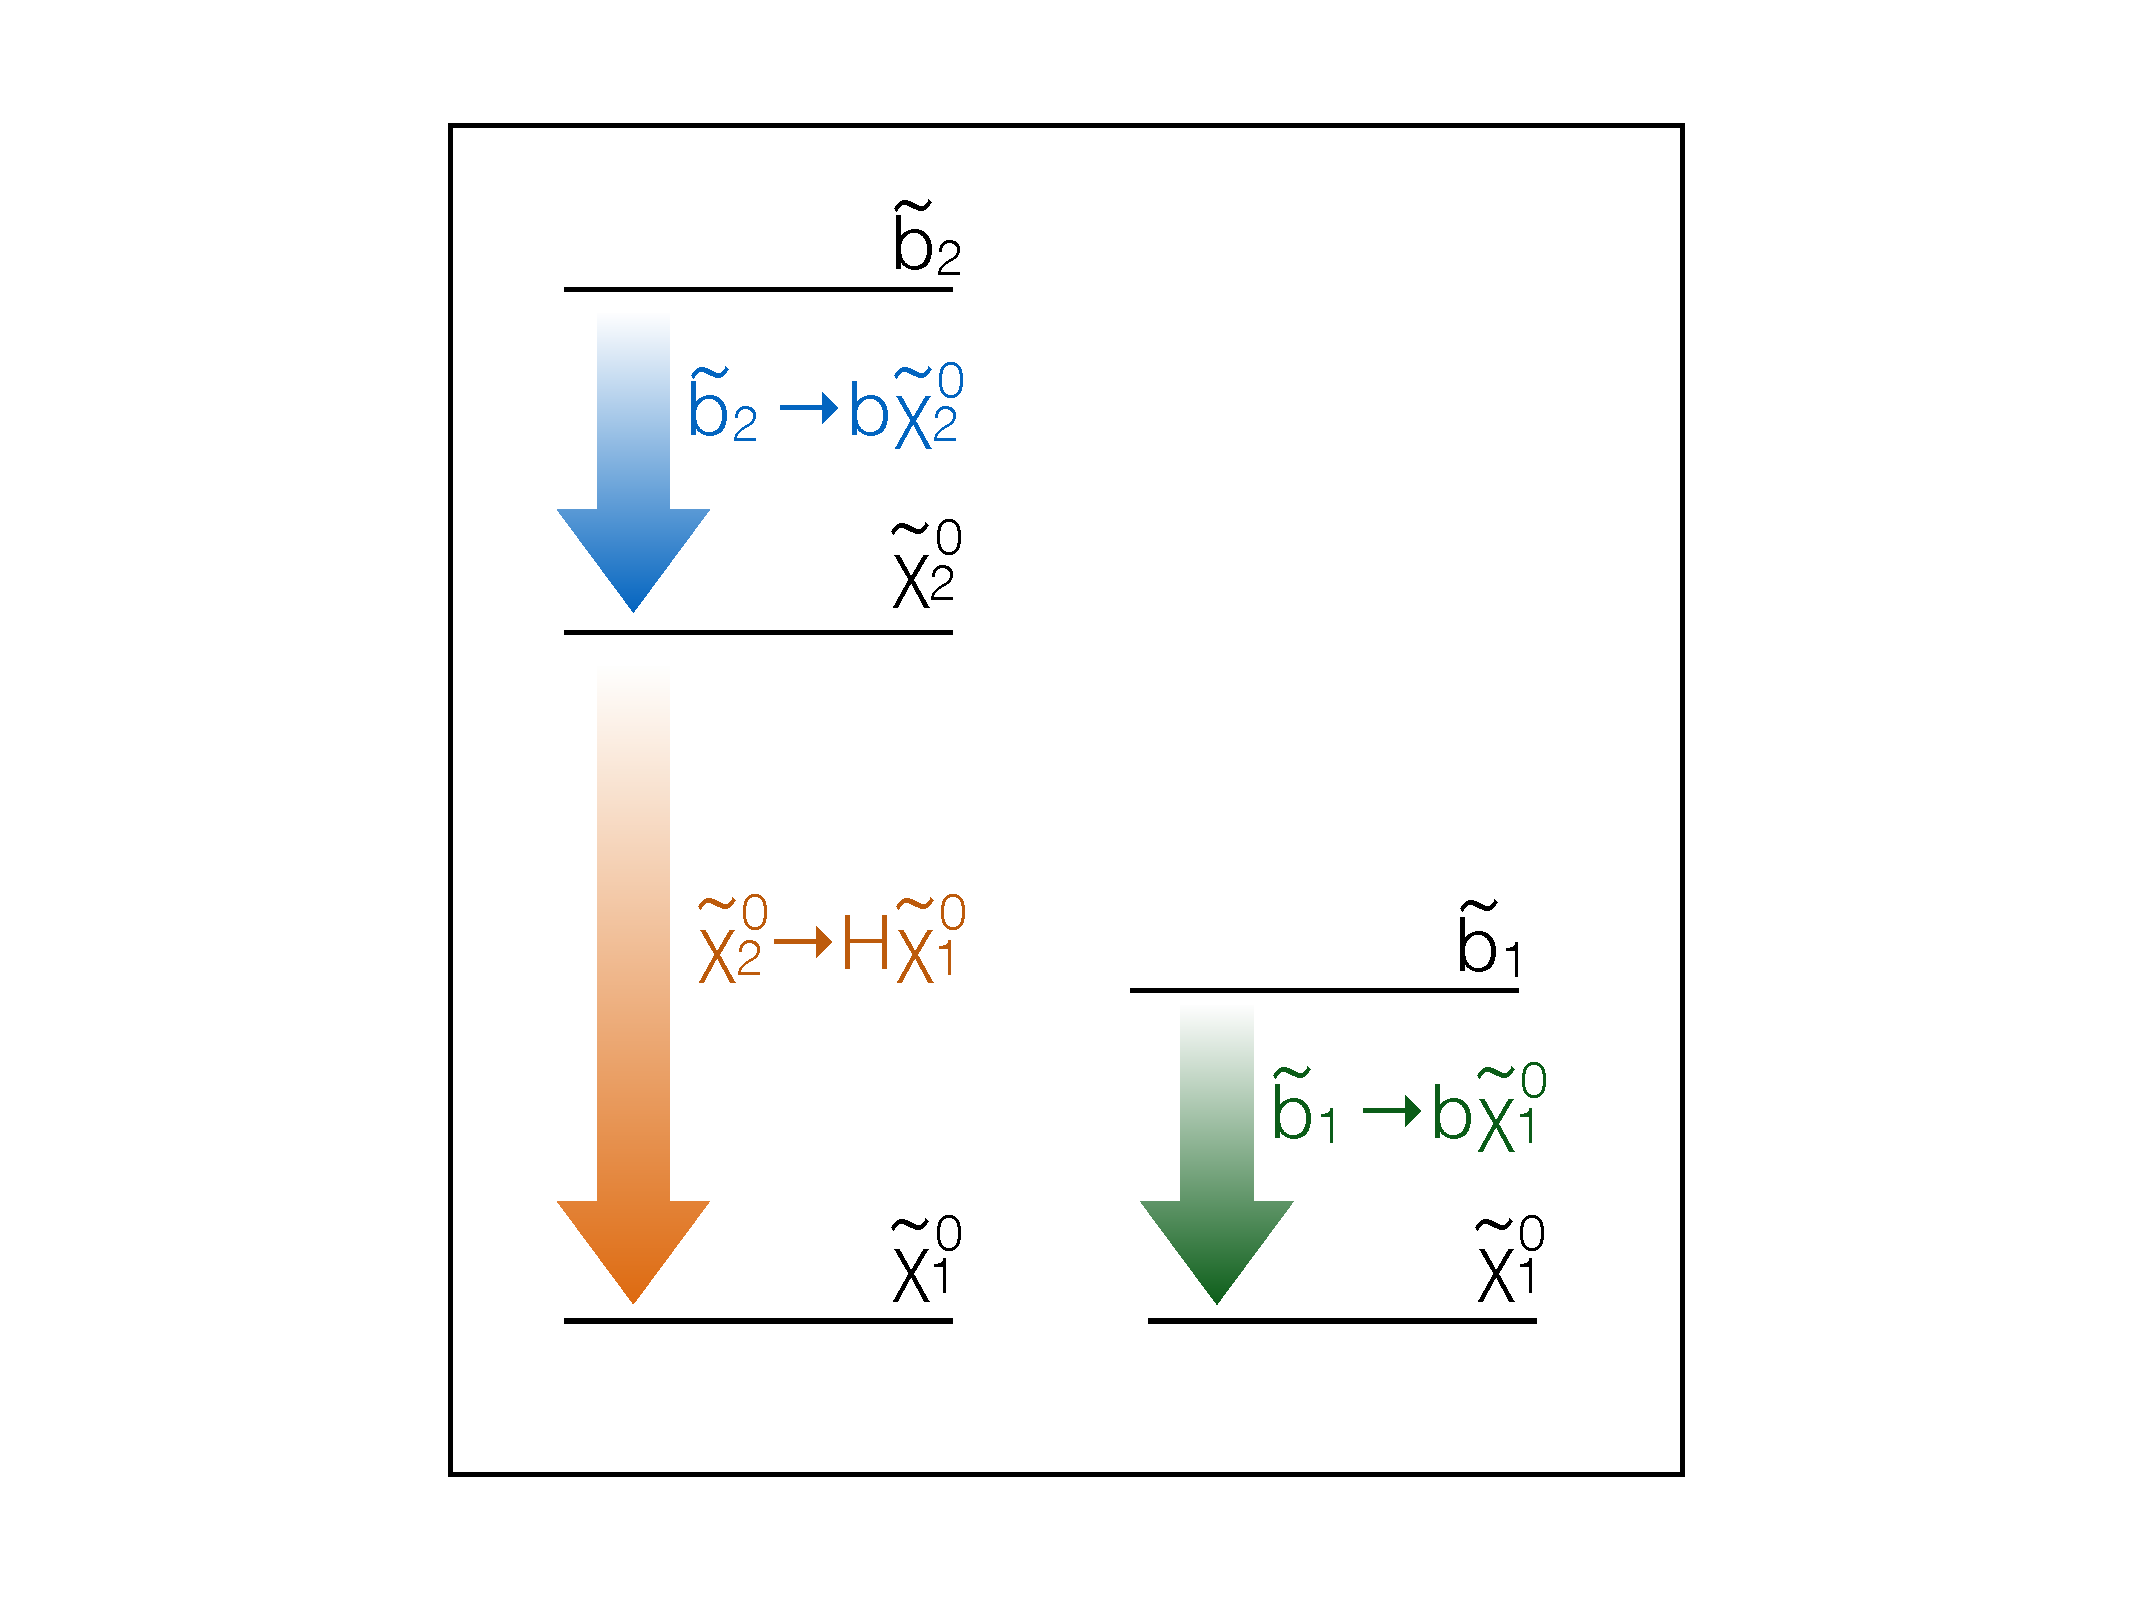
\includegraphics[width=0.23\textwidth,viewport=250 100 800 700,clip=true]{plots/model1}
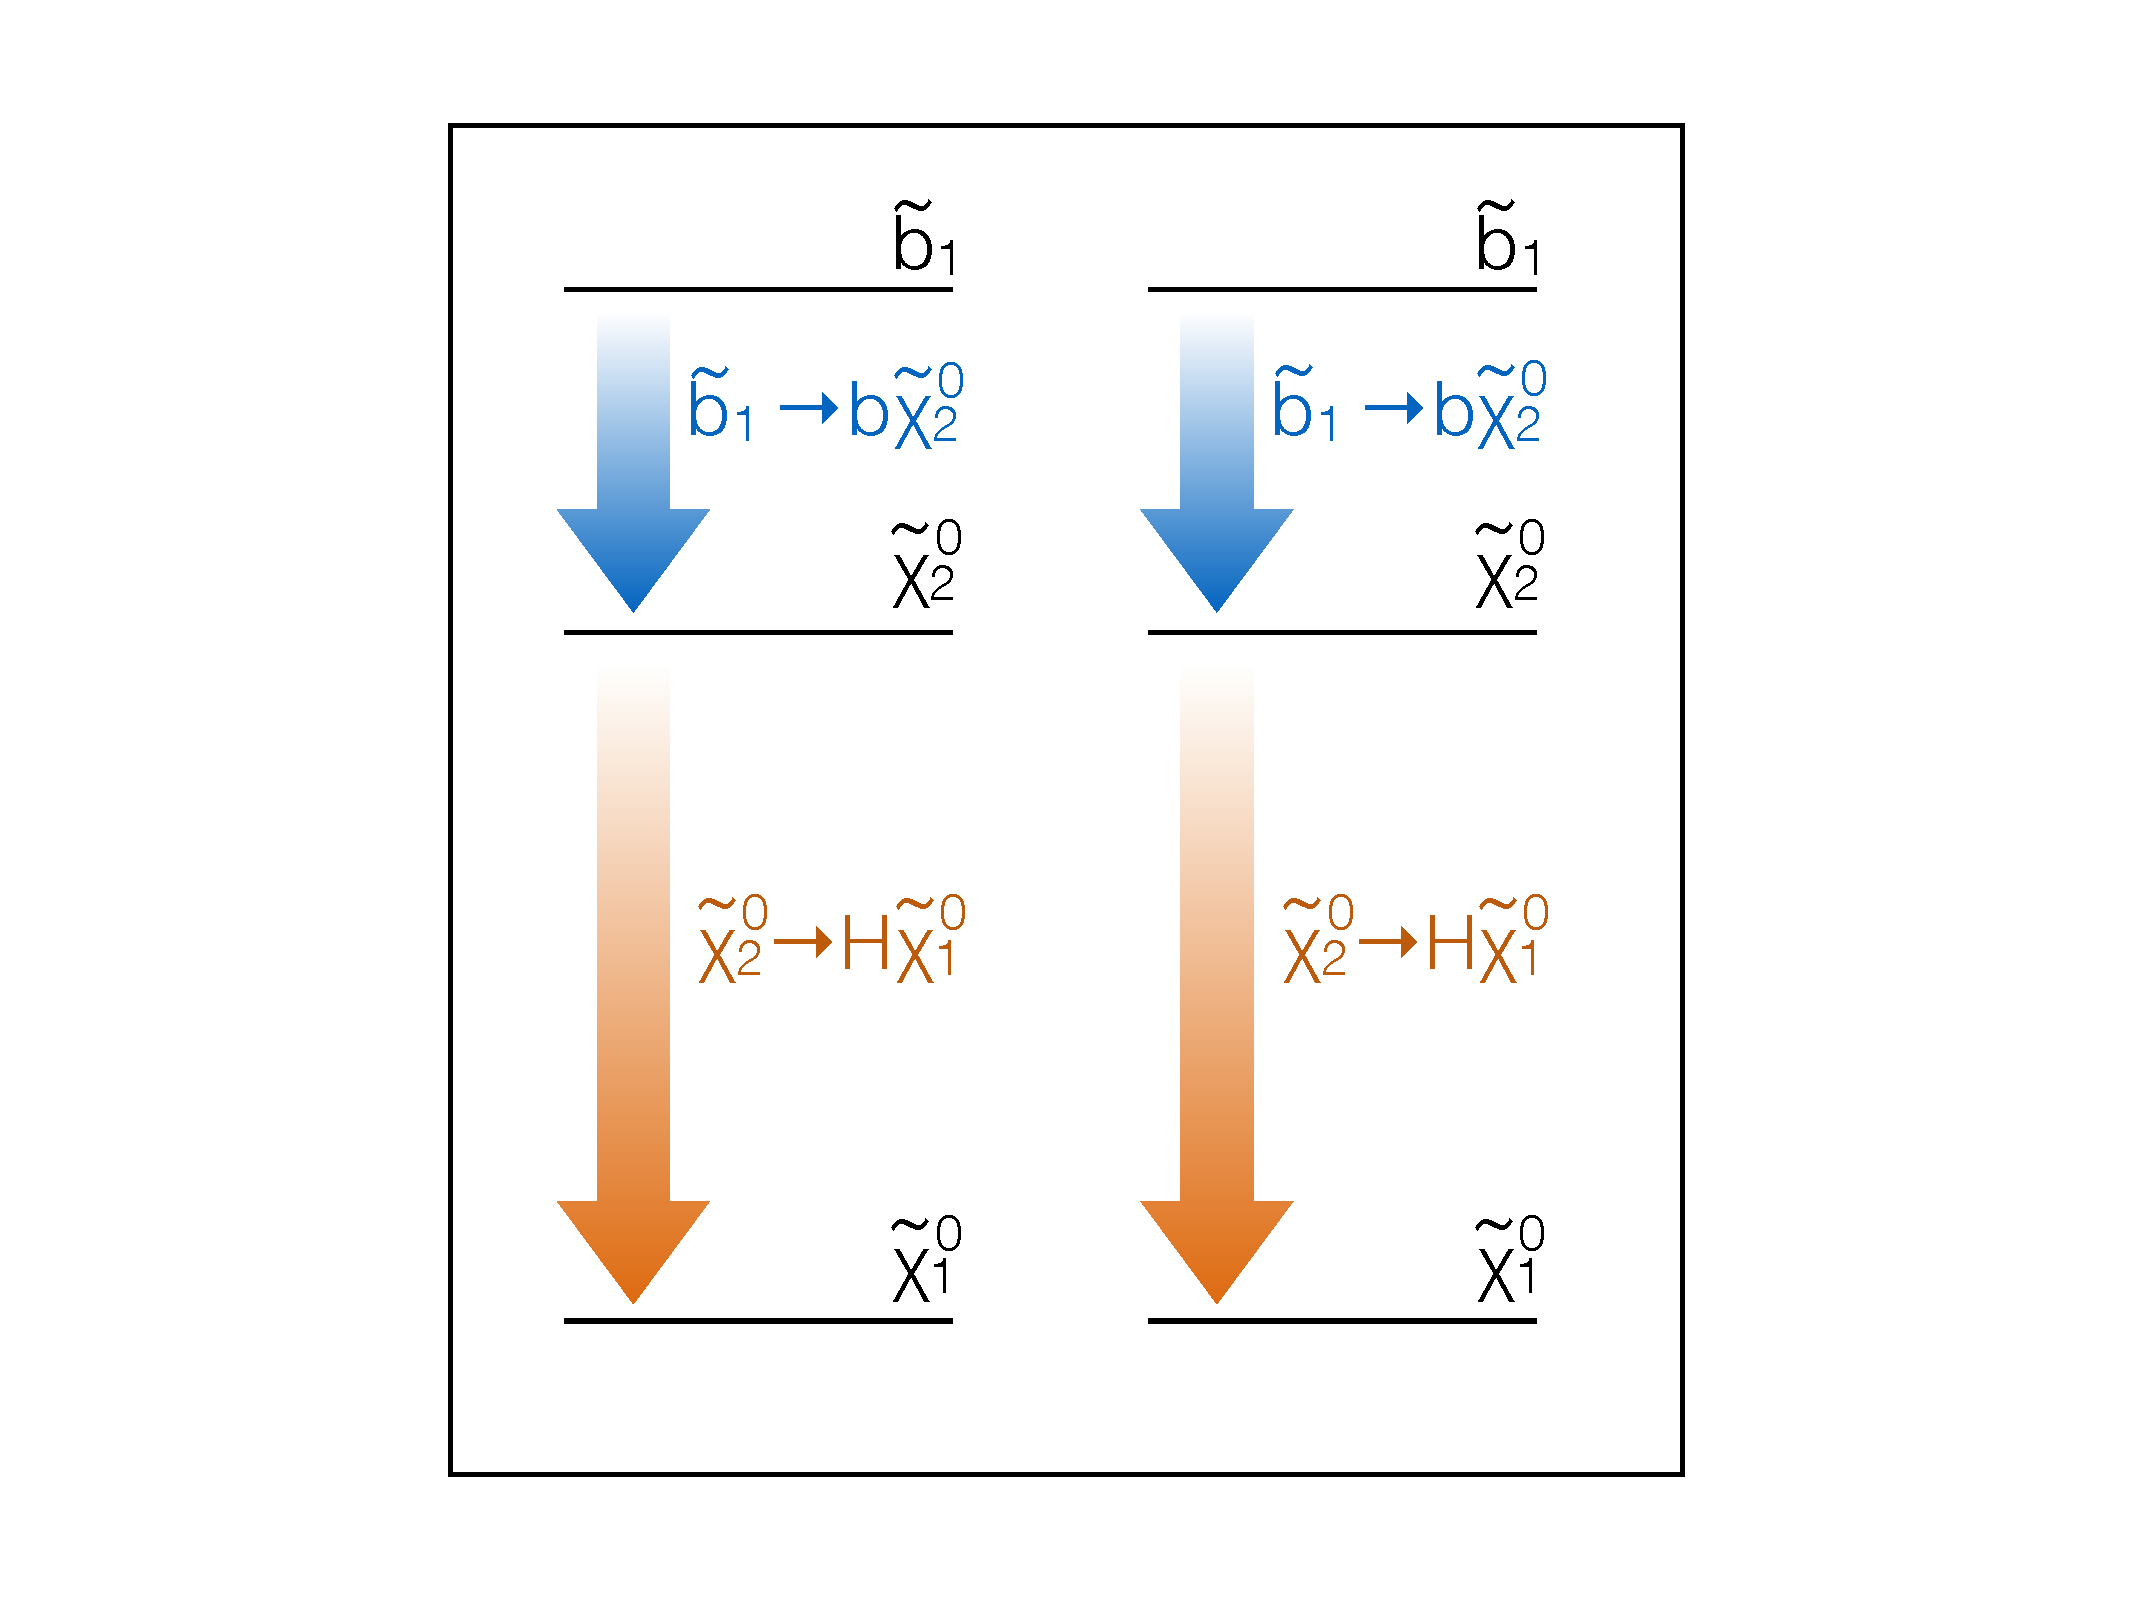
\includegraphics[width=0.23\textwidth,viewport=250 100 800 700,clip=true]{plots/model2}
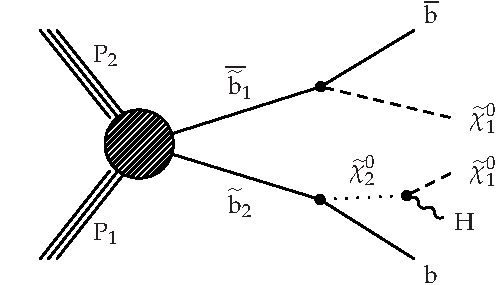
\includegraphics[width=0.23\textwidth]{plots/T21bH.pdf}
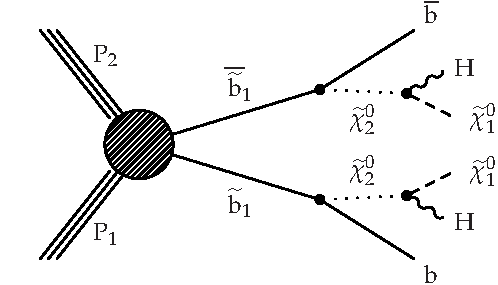
\includegraphics[width=0.23\textwidth]{plots/T2bH.pdf}
\caption{\label{fig:simplifiedModels} Pictorial representation of the
  decay chains and event topologies associated with model A (left) and model B (right), as described in the text.}
\end{figure}